\chapter{Implementation}
\label{chap:impl}
\begin{markdown}
  
# Introduction #

This chapter describes the implementation of the PTX.jl library
described in Section \ref{sec:meth:ptx}. The implementation consists
of three phases. __1)__ Creating a LLVM loadable module from a Julia
function, __2)__ lowering the function to code executable by a GPU and
__3)__ compiling the code into ptx. The first phase is implemented in
Julia as a __module generator__, and the last two are combined in a
__lowering compiler__. Figure \ref{fig:compiler} gives a overview of
the library.

The CUDA.jl library is used as a glue to transfer data to and from the
device and schedule the generated code on the device.

In this chapter, we will iterate through the design. First we look at
the implementation from an overview perspective, and then a simplified
flow through the pipeline. The last section will look at some
important implementation details.

# Overview #

\begin{figure}[H]
  \centering
  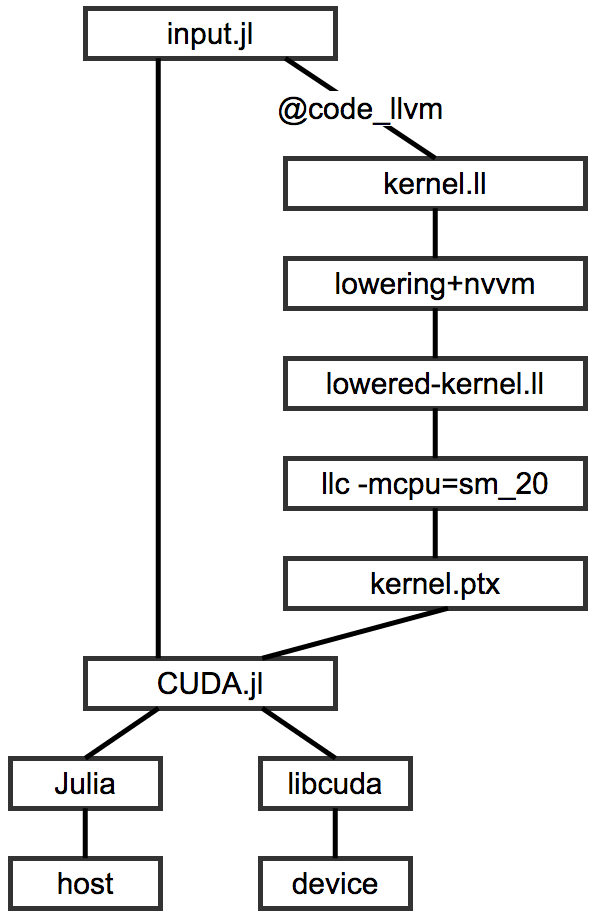
\includegraphics[width=200px]{body/figures/compiler.png}
  \caption{}
  \label{fig:compiler}
\end{figure}

Figure \ref{fig:compiler} illustrates the process of the code
generation. A julia function, adhering to the kernel language defined
in \ref{sec:meth:kernel}, is turned into LLVM IR by the module
generator. This code is then lowered into code that the LLVM PTX
backend can create code for. Here a modified version of the \gls{LLC}
is employed. The PTX code can then be loaded and executed into the GPU
with existing CUDA bindings written for Julia.

### Julia Module Generator ###

The module generator phase is responsible for producing a valid LLVM
_Module_. It is implemented on top of the Julia built-in
\textit{@code_llvm} macro. The interface to the generator is the
_code_module_ function.

### Lowering Compiler ###

The lowering compiler is built on top of the \gls{LLC}. The compiler
extends \gls{LLC} by linking to predefined libraries, and a lowering
and annotating compiler pass.

The interface to the library as a whole is a function called
_code_ptx_. It has the same signature as the function version of
_code_llvm_.

# A Guided tour through the compiler #

This section will go through the compiler step by step, looking at the
generated code to show how the code is transformed. Some details are
left out and discussed in Section \ref{sec:implementation-details}.


\begin{figure}[H]
  \begin{minted}[linenos,numbersep=5pt,gobble=2,frame=lines,framesep=2mm]{julia}
  function copy(from, to)
    i = get_global_id(0);
    to[i] = from[i];
  
    return
  end
  \end{minted}
  \caption{}
  \label{fig:julia-copy}
\end{figure}

Consider the Julia kernel function in Figure \ref{fig:julia-copy}. It
is transformed by executing the Julia statement in Figure
\ref{fig:impl:code_ptx}.

\begin{figure}[H]
  \begin{minted}[linenos,numbersep=5pt,gobble=2,frame=lines,framesep=2mm]{julia}
  code_ptx(copy, (GPUArray{Int64}, GPUArray{Int64}))
  \end{minted}
  \caption{Generating PTX from a Julia function}
  \label{fig:impl:code_ptx}
\end{figure}


## A LLVM module for Julia Function ##

The macro __@code\_llvm__ compiles a Julia function with arguments
down to the corresponding LLVM IR representation. In order to load
this string into a LLVM module, function declarations and types used
in the function must be included. As seen in Figure
\ref{fig:copy_llvm} the extra information need is included. 

\begin{figure}[H]
  \begin{minted}[linenos,numbersep=5pt,gobble=2,frame=lines,framesep=2mm]{llvm}
  %jl_value_t = type { %jl_value_t* }
     
  define void @copy(%jl_value_t*, %jl_value_t*) {
  top:
    %2 = call i64 @get_global_id(i64 0)
    %3 = call i64 @getindex(%jl_value_t* %0, i64 %2)
    %4 = call i64 @setindex(%jl_value_t* %1, i64 %3, i64 %2)
    ret void
  }
  
  declare i64 @setindex(%jl_value_t*, i64, i64)
  declare i64 @getindex(%jl_value_t*, i64)
  declare i64 @get_global_id(i64)
  \end{minted}
  \caption{}
  \label{fig:copy_llvm}
\end{figure}

## Lowering the code ##

The lowering LLVM pass transforms the function in figure
\ref{fig:copy_llvm} to the one in figure \ref{fig:copy_lowered}. In
this step, the GPU low level implementations for the arrays have been
linked and inlined, in place of the calls to __getindex__ and
__setindex!__ in Figure \ref{fig:copy_llvm}. The __get_global_id__
function has been mangled to enable it to be linked with its
implementation in the next step. The Julia arrays represented with
__jl_value_t__ has been replaced with an unboxed integer pointer in the
_global_ address space. The annotating pass has added the
__!nvvm.annontations__ named metadata, and it is set up so the PTX
backend recognizes the function as a kernel.

\begin{figure}[H]
  \begin{minted}[linenos,numbersep=5pt,gobble=2,frame=lines,framesep=2mm]{llvm}
  target datalayout = "e-p:32:32:32-i1:8:8-i8:8:8- ... -v1024:1024:1024"
  target triple = "nvptx64-nvidia-cuda"
  
  declare i64 @get_global_id(i32)
  
  define void @copy(i64 addrspace(1)*, i64 addrspace(1)*) {
  top:
    %2 = call i64 @get_global_id(i32 0)
    %3 = getelementptr inbounds i64 addrspace(1)* %0, i64 %2
    %4 = load i64 addrspace(1)* %3, align 8, !tbaa !2
    %5 = getelementptr inbounds i64 addrspace(1)* %1, i64 %2
    store i64 %4, i64 addrspace(1)* %5, align 8, !tbaa !2
    ret void
  }
  
  !llvm.ident = !{!0}
  !nvvm.annotations = !{!1}
  
  !0 = metadata !{metadata !"Apple LLVM version 6.0 (clang-600.0.54) (based on LLVM 3.5svn)"}
  !1 = metadata !{void (i64 addrspace(1)*, i64 addrspace(1)*)* @copy, metadata !"kernel", i32 1}
  \end{minted}
  \caption{}
  \label{fig:copy_lowered}
\end{figure}

## Compiling the code to PTX ##

The LLVM static compiler, __llc__, is used to compile the lowered LLVM
IR into PTX code. The code is now ready to be loaded into the GPU by
the existing CUDA libraries for Julia.

# Implementation details #
\label{sec:implementation-details}

This section discusses implementation details which were vital
to realize the PTX.jl library.

## Disabling inlining ##

A key to the method used in PTX.jl is to disable inlining. This can be
done in two ways, either extending the Julia compiler or tricking the
inlining mechanism.

### Compiler extension ###

The compiler extension is to create a macro, \textit{@noinline} analogous to
the existing \textit{@inline}. The macro annotates a method so that the Julia
inlining mechanism will not consider a call to the method for
inlining.

### The inline hack ###

The hack is to create a function, _noinline_, that does not get
inlined. This is done by examining the inlining mechanism in Julia, and
designing a function that is not subject to inlining.

By forcing this function to be inlined in the function, you do not want
inlined, you end up with a mechanism to avoid inlining. This is done
by annotating the _noinline_ function with the macro \textif{@inline}. This
bypasses the regular inline mechanism and will forcibly inline any
function.

### Choosing the hack ###

The latter approach is chosen to avoid changes to the compiler. This
hack might be temporary, as there are discussions involving the Julia
function _llvmcall_ that might enable the similar behavior in a more
clean way.

## Unboxed arrays ##
\label{sec:implementation-details-unboxed}

The unboxed array implementation is a shared implementation between
Julia and OpenCL C. On the Julia side, the type is represented by
__GPUArray__. The type is generic and is a vector of _Int32s_,
_Int64s_, _Float32s_ or _Float64s_. The methods for the __setindex!__
and __getindex__ functions are implemented as stubs for the vector
type in Julia. These are called when the element operator in Julia is
used. On the OpenCL C side, these functions are implemented over
unboxed arrays i.e. c pointers. 

## Function Lowering ##

The kernel function is lowered by substituting a Julia __GPUArray{T}__
with the LLVM IR \textbf{T*}. The replacement starts by lowering the
parameters of the kernel. Then the _use graph_ of the parameter in the
function is lowered. In addition, all calls to the Julia stubs are
linked against the OpenCL implementation. The OpenCL name mangling
rules are employed to support multiple primitive types (See Section
\ref{sec:impl:types}).

## Built-In kernel functions ##

As mentioned in Section \ref{sec:meth:built-ins}, the OpenCL
specification defines built-in functions that are available to a
kernel. __libclc__ \cite{libclc} provides an open source
implementation of the runtime library for the LLVM NVPTX backend. This
library is used \textit{as is} and is linked just before the
optimization phase so that the library functions can be inlined by the
LLVM optimizer.

## Supporting multiple primitive types ##
\label{sec:impl:types}

The implementation supports 32- and 64-bits integer and floating point
numbers. To facilitate this, the functions mentioned in
\ref{sec:implementation-details-unboxed} are overloaded for the four
types. Type information in Julia is contained inside the argument as a
runtime value. Therefore the information is not accessible by calling
the \textit{@code_llvm} macro, running at compile time. This is solved
by passing the type information in a named metadata node, added to the
module in the module generator. This implies that the kernel has a
fixed type and must be generated for each type.

## Inexpensive Linking ##

The linking functionality of \gls{LLVM} enables linking a module with
all the function implementations and definitions of another
module. This is not necessary for the kernel compiler, and running dead
code elimination after linking is not very performant. As a
consequence, the linking procedure from the \gls{pocl} \cite{pocl} compiler is
included and used when linking a kernel to the built-in definitions
exposed by libclc. The \gls{pocl} linker copies only the functions
that are in the call graph of functions in the original module, and
ignores functions that are not called.

\end{markdown}
